\section*{Úkol 3}
\label{sec:task-3}

Na hladině významnosti 5 \% rozhodněte, zda střední hodnoty (popř\. mediány) nárůstů FPS po aplikaci 1.5 patche statisticky významně závisí na typu grafické karty.
Posouzení proveďte nejprve na základě explorační analýzy a následně pomocí vhodného statistického testu, včetně ověření potřebných předpokladů.
V případě, že se nárůst FPS pro různé grafické karty statisticky významně liší, určete pořadí karet dle středního nárůstu FPS (popř\. mediánu nárůstu FPS).
\textbf{Poznámka:} \textit{Srovnání proveďte pro všechny čtyři typy grafických karet.}

\renewcommand{\skewnessValues}{-0.2, 0.2, 0.2, -0.4}
\renewcommand{\kurtosisValues}{-1.1, -1.0, -1.1, -0.7}
\renewcommand{\shapireWilk}   {0.012, 0.006, 0.005, 0.019}
\renewcommand{\symmetryTest}  {0.087, 0.218, 0.043, 0.016}

\renewcommand{\meanValues}{5.200, 5.700, 4.750, 5.300}
\renewcommand{\ttRtxValues} {4.950, 5.250, 5.600, 5.850}
\renewcommand{\ttAmdValues} {4.700, 4.900, 5.100, 5.345}
\renewcommand{\rtxDvaInterval} {(\tableValue{\ttRtxValues}{0}, \tableValue{\ttRtxValues}{1}) }
\renewcommand{\rtxTriInterval} {(\tableValue{\ttRtxValues}{2}, \tableValue{\ttRtxValues}{3}) }
\renewcommand{\amdSestInterval} {(\tableValue{\ttAmdValues}{0}, \tableValue{\ttAmdValues}{1}) }
\renewcommand{\amdSedmInterval} {(\tableValue{\ttAmdValues}{2}, \tableValue{\ttAmdValues}{3}) }

\begin{enumerate}[label=\alph*)]
    \item Daný problém vhodným způsobem graficky prezentujte (vícenásobný krabicový graf, histogramy, q-q grafy). 
    Srovnání okomentujte (včetně informace o případné manipulaci s datovým souborem).

    \newline{
        \begin{figure}[h!]
            \centering
            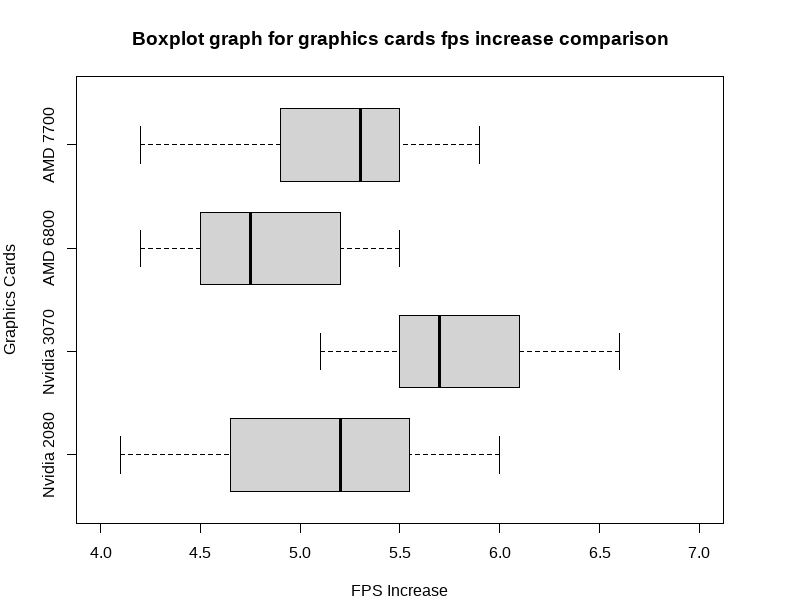
\includegraphics[width=0.75\textwidth]{assets/box_plot_all}
            \caption{Krabicový graf srovnávající nárůst FPS pro všechny čtyři grafické karty}
            \label{fig:box_plot_all}
        \end{figure}

        Pro další analýzu již použijeme data upravená o odlehlá pozorování. Dle \figref{fig:box_plot_all}, \figref{fig:histogram_all} a \figref{fig:qq_all} lze usuzovat, že nárůst FPS u grafické karty \nvidiaCardTri\ je výrazně vyšší než u ostatních grafických karet.

        \begin{figure}[h!]
            \centering
            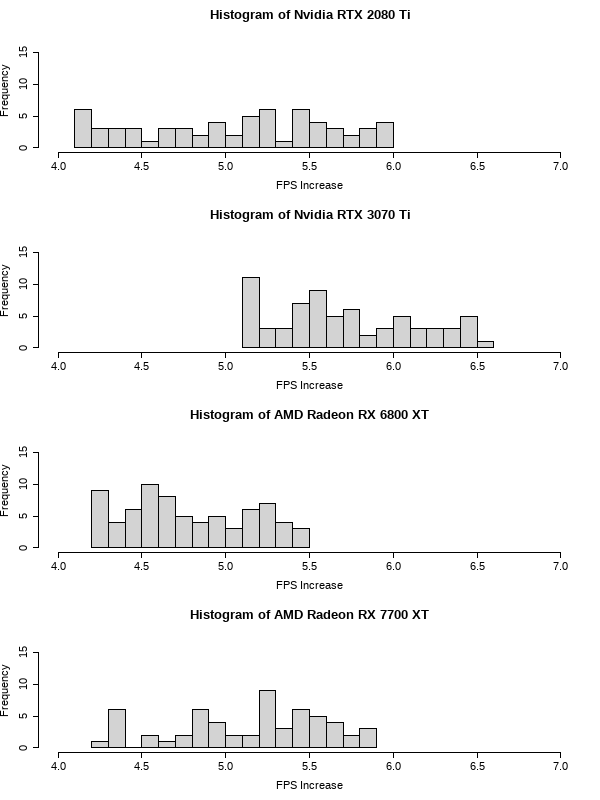
\includegraphics[width=0.75\textwidth]{assets/histograms_all}
            \caption{Histogramy srovnávající nárůst FPS pro všechny čtyři grafické karty}
            \label{fig:histogram_all}
        \end{figure}

        \begin{figure}[h!]
            \centering
            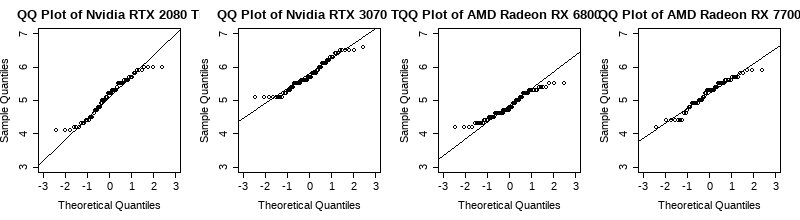
\includegraphics[width=1.0\textwidth]{assets/qq_all}
            \caption{Q-Q grafy srovnávající nárůst FPS pro všechny čtyři grafické karty}
            \label{fig:qq_all}
        \end{figure}
    }
    
    \newpage
    \item Ověřte normalitu a symetrii nárůstů FPS u všech čtyř grafických karet (empiricky i exaktně).

    \vspace{1em}
    \begin{minipage}{0.94\textwidth}
        Podle grafu Q-Q (viz \figref{fig:qq_all}), je viditelné, že nárůst FPS pro všechny grafické karty není v souladu s normálním rozdělením.
        Tomu ale neodpovídají hodnoty šikmosti a špičatosti, které se nacházejí v intervalu (-2, 2) (viz \tabref{tab:normality-test-all}).

        \vspace{1em}
        \captionof{table}{Ověření normality nárůstu FPS dle grafických karet}
        \label{tab:normality-test-all}
        \renewcommand{\arraystretch}{1.3}
        \resizebox{\textwidth}{!}{%
            \begin{tabular}{|p{5cm}|P{3.5cm}|P{3.5cm}|P{4cm}|P{4cm}|}
                \hline
                               & \textbf{šikmost}                & \textbf{špičatost}              & \textbf{Shapirův-Wilkův test (p-hodnota)} & \textbf{Test symetrie}        \\ \hline
                \nvidiaCardDva & \tableValue{\skewnessValues}{0} & \tableValue{\kurtosisValues}{0} & \tableValue{\shapireWilk}{0}              & \tableValue{\symmetryTest}{0} \\ \hline
                \nvidiaCardTri & \tableValue{\skewnessValues}{1} & \tableValue{\kurtosisValues}{1} & \tableValue{\shapireWilk}{1}              & \tableValue{\symmetryTest}{1} \\ \hline
                \amdCardSedm   & \tableValue{\skewnessValues}{2} & \tableValue{\kurtosisValues}{2} & \tableValue{\shapireWilk}{2}              & \tableValue{\symmetryTest}{2} \\ \hline
                \amdCardSest   & \tableValue{\skewnessValues}{3} & \tableValue{\kurtosisValues}{3} & \tableValue{\shapireWilk}{3}              & \tableValue{\symmetryTest}{3} \\ \hline
            \end{tabular}%
        }
        \vspace{1em}

        Dle Shapirova-Wilkova testu (viz \tabref{tab:normality-test-all}) nelze na hladině významnosti 0.05 nárust FPS u grafických karet považovat za normálně rozdělený.
        Z tohoto důvodu je nutné provést neparametrické testy. \\

        Po provedení testu symetrie, bylo zjištěno, že u grafických karet \nvidiaCardDva, \amdCardSedm a \amdCardSedm\ bylo zamítnuto symetrické rozdělení.
        A u grafické karty \nvidiaCardTri\ nebylo zamítnuto symetrické rozdělení. \\

        Proto v následující analýze budeme předpokládat, že nárůst FPS u všech grafických karet není symetrický.
    \end{minipage}

    \newpage
    \item Ověřte homoskedasticitu (shodu rozptylů) nárůstů FPS mezi jednotlivými kartami (empiricky i exaktně)

    \vspace{1em}
    \begin{minipage}{0.94\textwidth}
        Dle \figref{fig:box_plot_all} a výpočtu poměru největšího a nejmenšího rozptylu nárůstu FPS $(\frac{S^2_{max}}{S^2_{min}} \cong 2.3)$ se zdá, že srovnávané rozptyly nelze považovat za srovnatelné. \\

        Na základě Leveneho testu s výslednou p-hodnotou $0.006$ zamítáme předpoklad o shodě rozptylů nárůstu FPS mezi grafickými kartami.
    \end{minipage}
    
    \newpage
    \item Určete bodové a 95\% intervalové odhady střední hodnoty (popř\. mediánu) nárůstů FPS pro všechny srovnávané karty.
    Volbu charakteristik proveďte tak, aby byly v souladu se statistickým testem, který plánujete provést v bodě e). 
    (Nezapomeňte na ověření předpokladů pro použití příslušných intervalových odhadů.)

    \vspace{1em}
    \begin{minipage}{0.94\textwidth}
        Vzhledem k zamítnutí předpokladu o normalitě rozdělení nárůstů FPS mezi grafickými kartami použijeme Kruskalův-Wallisův test, který ověřuje shodu mediánů.
        Z tohoto důvodu využijeme mediány rovněž v rámci odhadu měr polohy.
        Pro určení intervalového odhadu byla použita Wilcoxonova statistika (viz \tabref{tab:interval-estimation-all}). \\

        Přestože její předpoklady (symetrie rozdělení) nejsou splněny, jedná se však o nejrobustnější test, který máme k dispozici.
        Jeho použití je tedy zvoleno s vědomím, že výsledky mohou být zkreslené a jejich interpretace by měla být prováděna obezřetně.

        \vspace{1em}
        \captionof{table}{Bodové a intervalové odhady mediánu nárůstů FPS dle grafických karet}
        \label{tab:interval-estimation-all}
        \vspace{0.5em}
        \renewcommand{\arraystretch}{1.3}
        \resizebox{\textwidth}{!}{%
            \begin{tabular}{|p{5cm}|P{6cm}|P{9cm}|}
                \hline
                                & \textbf{bodový odhad (FPS)} & \textbf{95\% levostranný intervalový odhad (FPS)} \\ \hline
                \nvidiaCardDva  & \tableValue{\meanValues}{0} & \rtxDvaInterval                                   \\ \hline
                \nvidiaCardTri  & \tableValue{\meanValues}{1} & \rtxTriInterval                                   \\ \hline
                \amdCardSest    & \tableValue{\meanValues}{2} & \amdSestInterval                                  \\ \hline
                \amdCardSedm    & \tableValue{\meanValues}{3} & \amdSedmInterval                                  \\ \hline
            \end{tabular}%
        }
        \vspace{1em}

        U poloviny testovacích cyklů nárůst FPS nepřekročil \tableValue{\meanValues}{0} FPS pro grafickou kartu \nvidiaCardDva.\@
        95\% intervalový odhad mediánu nárůstu FPS pro tuto grafickou kartu je \rtxDvaInterval\.\@ \\

        U poloviny testovacích cyklů nárůst FPS nepřekročil \tableValue{\meanValues}{1} FPS pro grafickou kartu \nvidiaCardTri.\@
        95\% intervalový odhad mediánu nárůstu FPS pro tuto grafickou kartu je \rtxTriInterval\.\@ \\

        U poloviny testovacích cyklů nárůst FPS nepřekročil \tableValue{\meanValues}{2} FPS pro grafickou kartu \amdCardSest.\@
        95\% intervalový odhad mediánu nárůstu FPS pro tuto grafickou kartu je \amdSestInterval\.\@ \\

        U poloviny testovacích cyklů nárůst FPS nepřekročil \tableValue{\meanValues}{3} FPS pro grafickou kartu \amdCardSedm.\@
        95\% intervalový odhad mediánu nárůstu FPS pro tuto grafickou kartu je \amdSedmInterval\.\@ \\

        Na grafické kartě \amdCardSest\ můžeme pozorovat nejnižší medián nárůstu FPS, který se oproti \nvidiaCardDva\ a \amdCardSedm\ liší o cca 0.450 FPS.\@
        Pro grafickou kartu \nvidiaCardTri\ je medián nárůstu FPS nejvyšší, a to o cca 0.400 FPS oproti oproti kartám \nvidiaCardDva\ a \amdCardSedm\!.
        Ty se od sebe liší zhruba o 0.100 FPS.\@
    \end{minipage}

    \newpage
    \item Čistým testem významnosti ověřte, zda je pozorovaný rozdíl středních hodnot (popř\. mediánů) nárůstů FPS statisticky
    významný na hladině významnosti 5\%.\@
    Pokud ano, zjistěte, zda lze některé skupiny karet označit (z hlediska nárůstů FPS) za homogenní, tj\. určete pořadí karet dle středních hodnot (popř\. mediánů) nárůstů FPS.\@
    (Nezapomeňte na ověření předpokladů pro použití zvoleného testu.) \\

    \begin{minipage}{0.94\textwidth}
        Na hladině významnosti 0.05 zamítáme hypotézu o shodě mediánů nárůstu FPS mezi grafickými kartami (Kruskalův-Wallisův test, p-hodnota $\ll 0.001$).
        Tzn.\ mediány nárůstu FPS se mezi grafickými kartami statisticky významně liší. \\

        Test byl proveden i přes to, že předpoklady (symetrie rozdělení) nejsou splněny, jedná se však o nejrobustnější test, který máme k dispozici.
        Jeho použití je tedy zvoleno s vědomím, že výsledky mohou být zkreslené a jejich interpretace by měla být prováděna obezřetně. \\

        Pro určení, které skupiny karet lze označit za homogenní, jsme použili Dunnův test s Bonferroniho korekcí (viz. \tabref{tab:post-hoc-test}).

        \vspace{1em}
        \captionof{table}{Efekty nárůstu FPS dle grafických karet}
        \label{tab:post-hoc-test}
        \vspace{0.5em}
        \renewcommand{\arraystretch}{1.3}
        \resizebox{\textwidth}{!}{%
            \begin{tabular}{|p{5cm}|P{15cm}|}
                \hline
                               & \textbf{Efekt} \\ \hline
                \nvidiaCardTri & $0.400$        \\ \hline
                \amdCardSedm   & $0$            \\ \hline
                \nvidiaCardDva & $-0.100$       \\ \hline
                \amdCardSest   & $-0.550$       \\ \hline
            \end{tabular}%
        }

        \vspace{1em}
        \captionof{table}{Adjustované p-hodnoty post-hoc analýzy}
        \label{tab:letter-test}
        \vspace{0.5em}
        \renewcommand{\arraystretch}{1.3}
        \resizebox{\textwidth}{!}{%
            \begin{tabular}{|p{5cm}|P{4cm}|P{4cm}|P{4cm}|P{4cm}|}
                \hline
                               & \nvidiaCardTri & \amdCardSedm   & \nvidiaCardDva & \amdCardSest   \\ \hline
                \nvidiaCardTri & -              & \lowerThanZero & \lowerThanZero & \lowerThanZero \\ \hline
                \amdCardSedm   & \lowerThanZero & -              & 1.000          & \lowerThanZero \\ \hline
                \nvidiaCardDva & \lowerThanZero & 1.000          & -              & 0.008          \\ \hline
                \amdCardSest   & \lowerThanZero & \lowerThanZero & 0.008          & -              \\ \hline
            \end{tabular}%
        }
        \vspace{1em}

        Na hladině významnosti 0.05 byly nalezeny 3 homogenní skupiny (viz \tabref{tab:letter-test}), které se statistiky významně liší.
        Z výsledků post-hoc analýzy můžeme konstatovat, že nárůst FPS u grafické karty \amdCardSest\ je statisticky významně nižší než u zbylých grafických karet. \\

        Skupiny:
        \begin{enumerate}
            \item \nvidiaCardTri\ \\ - Efekt = $(0.400)$
            \item \amdCardSedm\ a \nvidiaCardDva\ \\ - Efekt = $<-0.100, 0>$
            \item \amdCardSest\ \\ - Efekt = $(-0.550)$
        \end{enumerate}
    \end{minipage}
\end{enumerate}

\endinput